\section{PROPENSITY SCORE MATCHING IN ACCOUNTING RESEARCH}

\paragraph{会計研究における PSM の利用 (Table 1 Panel A)}

\begin{table}
 \centering
 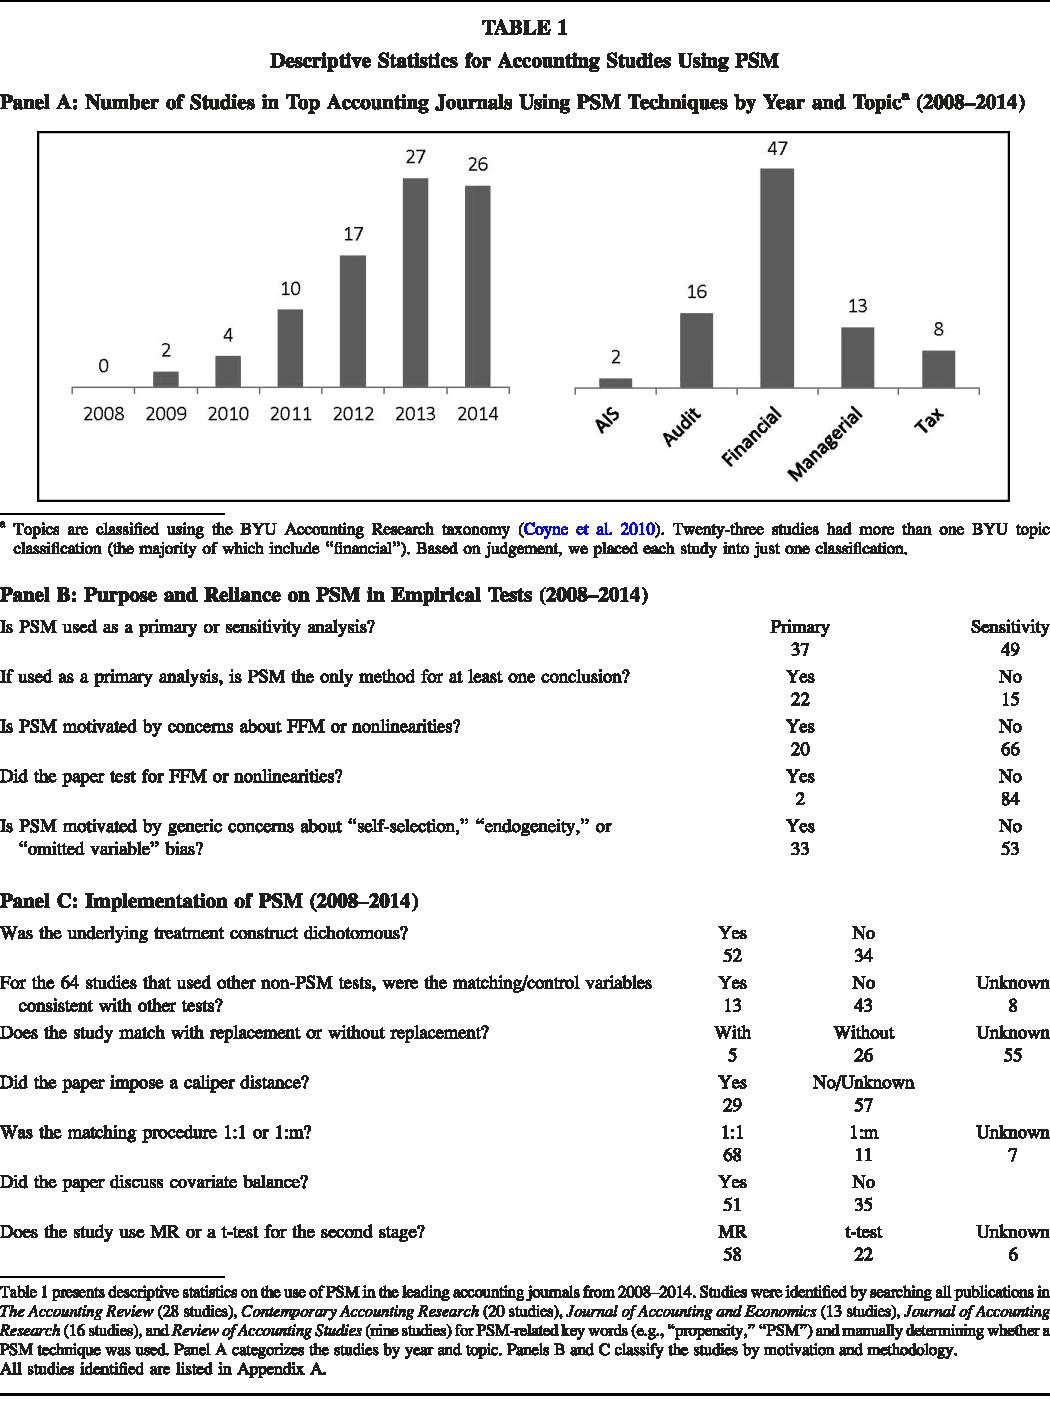
\includegraphics[width=14cm]{../table/tbl01.pdf}
\end{table}

\begin{itemize}
 \item 2008 $\sim$ 2014 年における、\textit{The Accounting Review,
       Contemporary Accounting Research, Journal of Accounting and
       Economics, Journal of Accounting Research, and Review of
       Accounting Studies} に掲載された論文延べ 86 件が対象。
 \item 会計研究で PSM が用いられはじめたのは最近 (86 件中 70 件は 2012
       $\sim$ 2014 の期間に刊行)。
\end{itemize}

\paragraph{各研究の PSM の位置付け (Table 1 Panel B)}

\begin{itemize}
 \item 主要な分析 (primary analyses) として用いている研究が 37 件である
       のに対し、ロバスト・チェック (sensitivity or robustness tests) と
       して用いている研究は 49 件。
 \item PSM を採用する理由として FFM や重回帰分析の線形性の仮定を挙げてい
       る研究はわずか 20 件。
 \item PSM が対処しうる内生性の問題を提示することなく、広く ``自己選択
       (self--selection),'' ``内生性 (endogeneity),'' および ``欠落変数
       バイアス (omitted variable bias)'' への対応として PSM を用いてい
       る研究が 33 件ある。
 \item Heckman (1979) の代わりとして誤用してしまっている研究も存在する。
\end{itemize}